%SOURCE : https://github.com/Gp2mv3/Syntheses
\documentclass[en]{sourcefiles/eplexam} % For a master exam in English, replace fr by en

%\usepackage{sourcefiles/eplcode} % Si l'examen contient du code. La commande pour insérer du code est \begin{lstlisting} ou pour un fichier \lstinputlisting{nomDeFichier}
%\lstset{language={Oz}, morekeywords={for,do,lazy}} % exemple de réglage avec Oz

\graphicspath{{img/}}

\hypertitle{Power Electronics}{8}{ELEC}{2660}{2022}{June}{All} % Remplacer Majeure par All si ce n'est pas un cours à option
{Maxime Leurquin}
{Marc Bekemans}

%Ce template a pour but de faciliter la rédaction des examens destinés à être posté sur Github. Cependant, il ne peut être posté sans respecter la hiérarchie établie dans le dossier du drive. Il est donc nécessaire de passer par un administrateur du drive (contact.epldrive@gmail.com), ou en suivant les instructions détaillées dans le fichier "How_to_Contribute" sur https://github.com/Gp2mv3/Syntheses. Notez qu'il est possible de contribuer de diverses manières!


%La ligne suivante est à supprimer à la compilation! Cette ligne crée une erreur, mais a été ajoutée afin d'éviter qu'overleaf ne mette du rouge partout.
\begin{document}

\noindent We had 2h to answer everything. There was no project this year. The exam was closed book. We could answer in english or french.

\section{}
For a flyback DC/DC converter: (4 points)
\begin{enumerate}

    \item Draw the electrical diagram with a snubber.

    \item Explain the role and the principle of operation of the snubber.
\end{enumerate}
\nosolution


\section{}
Explain the principle of operation of the Thyristor (2 points)

\nosolution


\section{}
In a peak current control, the duty-cycle is limited. Why? (3 points)
\nosolution


\section{}
We connect a rectifier on a 50Hz - three phase generator. On the AC side, the voltage between phases and neutral is 220V. The rectifier is connected to a capacitor on the DC side. (3 points)

\begin{enumerate}
    \item Draw the electrical circuit.
    \item What is the DC voltage after the rectifier in no load condition (only the capacitor connected).
\end{enumerate}

\nosolution



\section{}
We connect a single phase inverter supplied with 400V-DC voltage to a 220V 50Hz AC source through an inductance of 1mH.
What is the maximum active power transferable to the AC line? (3 points)

\nosolution


\section{}
For a DC/DC converter whose output capacitor is a 500µF and which has a voltage regulator bandwidth of 3kHz: (3 points)

\begin{enumerate}
    \item Represent on a bode diagram the shape of the output impedance (don't forget to scale the axes).
    
    \item Represent quantitatively (approximate) the time evolution of $V_{out}$ after an instantaneous load variation of 10A (Don't forget to scale the axes).
\end{enumerate}

\nosolution


\section{}
To which component does the construction scheme in figure \ref{fig:IGBT} correspond? Justify your answers. (2 points)

\begin{figure}[h]
    \centering
    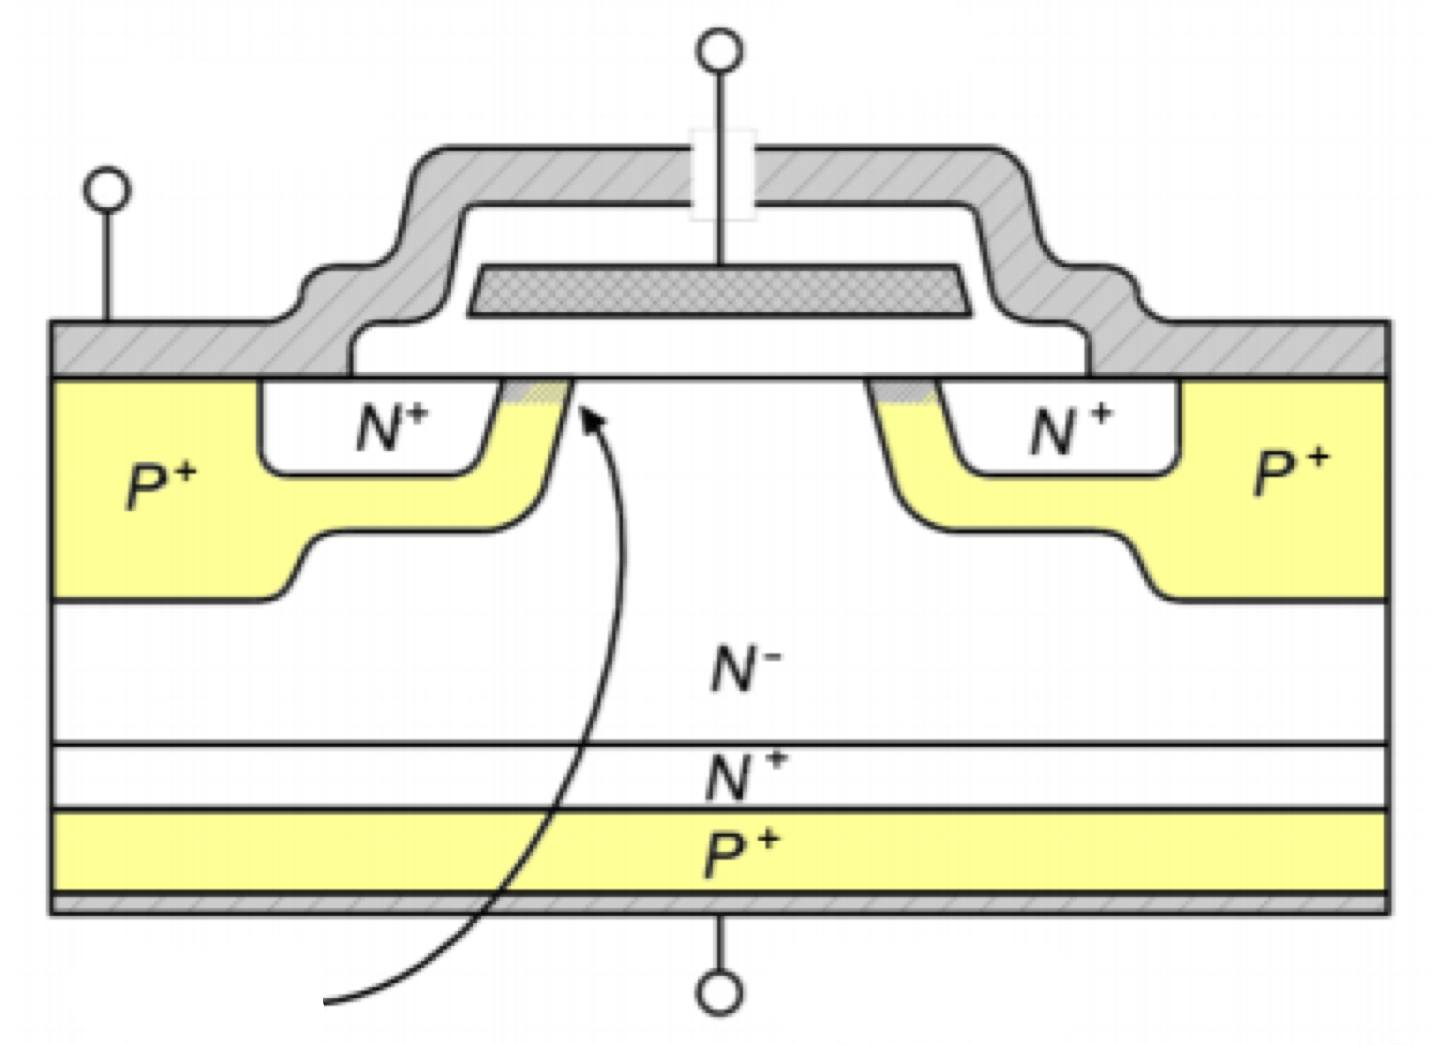
\includegraphics[width=0.5\textwidth]{IGBT.jpg}
    \caption{Construction scheme}
    \label{fig:IGBT}
\end{figure}


\begin{solution}
It is an IGBT.
\end{solution}

\end{document}


